% DRAFT generated from the testbed analysis summaries. Suggested text only;
% the author decides what enters the paper. Figures: figures/testbed/*.pdf.
\section{Experimental Results}

This section evaluates DIAS on a multi-machine testbed in terms of recommendation quality, adversarial failure, latency and throughput of the whole system and of each component, and resource use over time.

\subsection{Testbed Setup and Data Preparation}

Fig.~\ref{fig:tb-layout} shows the testbed. Four Linux virtual machines (M1--M4), each with three virtual CPUs and 6~GB of memory, run on one Apple M3 Max computer with 16 cores and 64~GB of memory. Docker Swarm joins the four Docker engines, and every container reaches the others through one overlay network. M1, M2, and M3 host the five organizations' peers with their CouchDB state databases, one Raft orderer each, and the six certificate authorities. M4 hosts the application backend, the load generator, and the Prometheus monitor. The Mac itself (M5) serves the language model on its GPU, because the MLX runtime needs that GPU.

The network runs Hyperledger Fabric~2.5.16 with the same block settings as the prototype: a block closes after 2~s or 10 transactions. The chaincode requires endorsement by three of the five organizations. The ledger records each request and each auditor decision together with the LLM recommendation value; the justification and the model's explanation stay off the ledger. Every 5~s, Prometheus records the CPU and memory of each machine, and a sampler records those of every container through the Docker statistics interface. The model machine is sampled on the Mac itself.

The recommendation data come from a seeded generator (seed 20260912) that applies the written policy through an offline reference oracle. It produced 10,513 raw examples, of which 8,013 form eight disjoint sets: 5,254 balanced training examples, 400 validation examples, five test sets of 600, 540, 389, 400, and 370 examples, and 60 workflow examples. No scenario family, fact set, or prompt of the training set appears in any test set. V7 fine-tunes Qwen3-14B (4-bit) with a rank-8 LoRA adapter on 16 layers for 5,254 iterations, with batch size 1, gradient accumulation 4, learning rate $10^{-5}$, and a maximum sequence length of 2,560 tokens.

For the system experiments, the ledger holds 120 users: the 20 users of the prototype and 100 load-test users that copy the twelve requester profiles, together with 3 cases and 20 case files covering all record types, sensitivity levels, and protection flags. Every request of every run is fixed in advance by a seeded plan that also stores the policy's answer to it, and no two requests in a run share the same verified facts. In every approval/deny workflow, the auditor follows the recommendation as soon as it appears; the reported times therefore contain no human review time.
\begin{figure*}[tb]
  \centering
  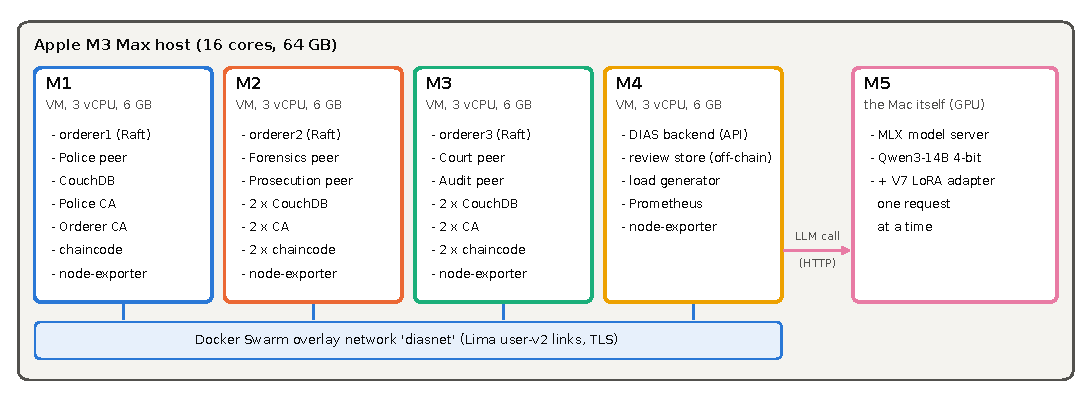
\includegraphics[width=\textwidth]{figures/testbed/testbed_layout.pdf}
  \caption{Multi-machine testbed.}
  \label{fig:tb-layout}
\end{figure*}

\subsection{Recommendation Quality}

Fig.~\ref{fig:tb-quality} shows where the 600 balanced test decisions end up for each model. Of the 300 requests that the policy allows, V7 recommends 298 for approval and wrongly refuses 2, whereas the untuned model approves only 70, refuses 204, and gives 26 unusable answers. Of the 300 requests that the policy denies, V7 denies 294 and wrongly grants 6; the untuned model denies 266, grants 14, and gives 20 unusable answers.

Table~\ref{tab:tb-quality} lists the same outcomes as counts. A usable answer is one the auditor screen can display; V7 gives 600 of 600 and the untuned model 554. A wrongly granted request is a security risk and a wrongly refused one costs the requester time, which is why both rows are reported separately. The correct reason code tells the auditor which rule decided the case, and the correct clause list points to the exact policy text the auditor must check: V7 names the right reason in 584 cases and the exact clauses in 572, against 203 and 130 for the untuned model.

On the same 600 cases, V7 is correct where the untuned model is wrong 264 times, and the reverse happens 8 times. An exact McNemar test on these paired decisions gives $p = 1.8e-67$, so the difference is not a chance effect of this test set.
\begin{figure}[tb]
  \centering
  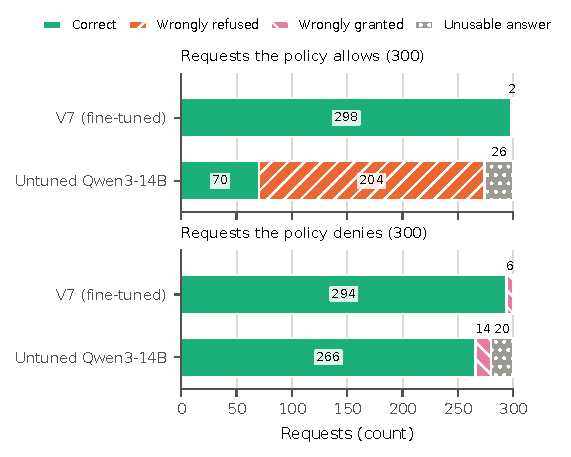
\includegraphics[width=\columnwidth]{figures/testbed/e1_outcomes_counts.pdf}
  \caption{Recommendation outcomes on 600 test decisions.}
  \label{fig:tb-quality}
\end{figure}
\begin{table}[tb]
  \centering
  \caption{Recommendation Outcomes on 600 Test Decisions}
  \label{tab:tb-quality}
  \footnotesize
  \begin{tabular}{@{}lrr@{}}
    \toprule
    Outcome & Untuned & V7 \\
    \midrule
    Usable answers (of 600) & 554 & 600 \\
    Allowed requests approved (of 300) & 70 & 298 \\
    Denied requests denied (of 300) & 266 & 294 \\
    Wrongly granted & 14 & 6 \\
    Wrongly refused & 204 & 2 \\
    Correct decisions (of 600) & 336 & 592 \\
    Correct reason code (of 600) & 203 & 584 \\
    Correct clause list (of 600) & 130 & 572 \\
    \bottomrule
  \end{tabular}
\end{table}

Table~\ref{tab:tb-sets} repeats the comparison on every held-out set. V7 is correct on at least 98.4\% of the cases of each set, including the paraphrased requests whose wording differs from training, whereas most errors of the untuned model are wrong refusals and unusable answers.
\begin{table}[tb]
  \centering
  \caption{Correct Decisions on Every Held-Out Set}
  \label{tab:tb-sets}
  \footnotesize
  \setlength{\tabcolsep}{3pt}
  \begin{tabular}{@{}lrrrr@{}}
    \toprule
    Set & Cases & Untuned & V7 & V7 wrongly granted \\
    \midrule
    Validation (balanced) & 400 & 215 & 395 & 3 \\
    Test, balanced decisions & 600 & 336 & 592 & 6 \\
    Test, balanced reasons & 540 & 448 & 536 & 4 \\
    Test, adversarial & 389 & 188 & 383 & 6 \\
    Test, paraphrased & 400 & 240 & 395 & 4 \\
    Test, several rules & 370 & 352 & 370 & 0 \\
    \bottomrule
  \end{tabular}
\end{table}

\subsection{Adversarial Failure Test}

Fig.~\ref{fig:tb-adversarial} shows the 204 adversarial requests that the policy denies and whose justifications contradict the facts or carry injected instructions. V7 stops 198 of them and wrongly grants 6, a rate of 2.94\% with a 95\% Wilson interval of 1.35--6.27\%. The untuned model grants 4 but cannot answer 25 of them at all, and it refuses 141 of the 185 allowed adversarial requests, so its lower count comes from denying almost everything. The failures of V7 remain the reason why the auditor, not the model, makes the binding decision.
\begin{figure}[tb]
  \centering
  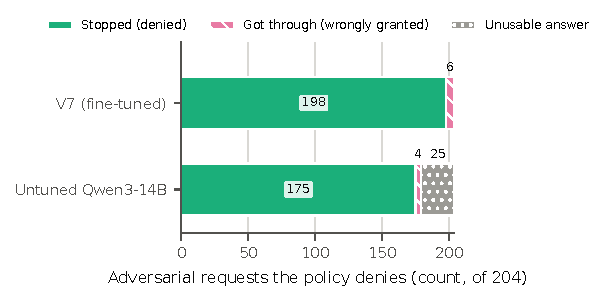
\includegraphics[width=\columnwidth]{figures/testbed/e2_adversarial_counts.pdf}
  \caption{Adversarial requests that the policy denies.}
  \label{fig:tb-adversarial}
\end{figure}

% Dynamic Authorization Reuse: keep the existing subsection; it was not re-run on the testbed.

\subsection{Latency and Throughput}
Fig.~\ref{fig:tb-components} splits the time of one approval/deny workflow into its components at 10, 25, 50, 75, and 100 simultaneous users; each level ran three times, and all 780 of 780 workflows completed. Panel (b) shows the work each workflow needs: the request commit, the LLM inference, the decision commit, and the application steps. This work stays between 9.61~s and 9.94~s at every level. The LLM inference takes 7.33~s, and the decision commit takes 2.05~s because a decision arrives alone and waits for the 2~s block timeout. The request commit grows from 0.10~s at 10 users to 0.42~s at 100: endorsement takes 0.05~s and 0.17~s, and the wait for the block 0.05~s and 0.24~s, far below the 2~s timeout because simultaneous requests fill blocks of ten transactions. Panel (a) shows that the wait for the single model server is what grows: from 34.0~s at 10 users to 363.5~s at 100.
\begin{figure}[tb]
  \centering
  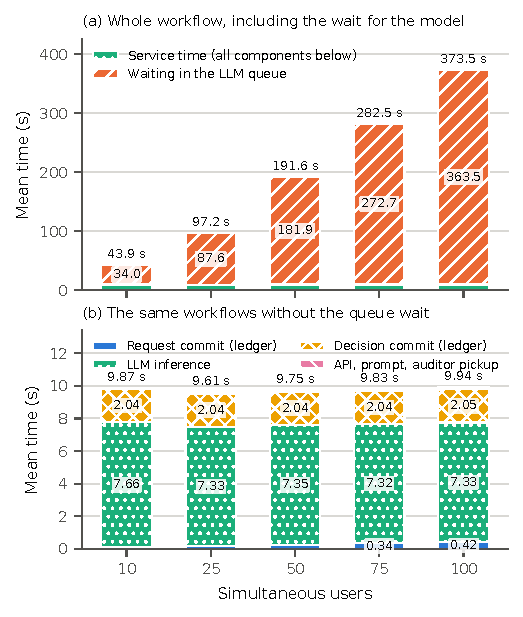
\includegraphics[width=\columnwidth]{figures/testbed/e5_components_by_users.pdf}
  \caption{Workflow time by component.}
  \label{fig:tb-components}
\end{figure}
Fig.~\ref{fig:tb-latency} plots the median and 95th-percentile workflow times. The median rises from 40.5~s at 10 users to 372.3~s at 100, and the 95th percentile from 77.7~s to 699.8~s. The median grows linearly with the number of users, by 3.69~s per additional user ($R^2 = 1.000$), because each additional request joins the same queue. Throughput stays between 7.62 and 8.16 completed workflows per minute (Fig.~\ref{fig:tb-throughput}); the model alone produces 7.27 recommendations per minute; adding users adds waiting, not completed work. The recommendations given under load agree with the written policy in 759 of 780 cases. Of the 21 disagreements, 7 wrongly grant and 14 wrongly refuse, and 19 concern the annotate action.
Replaying the 21 disagreeing requests one at a time with no other load gives the same decision in 21 cases and the identical model output in 21, so the errors do not come from the load.
\begin{figure}[tb]
  \centering
  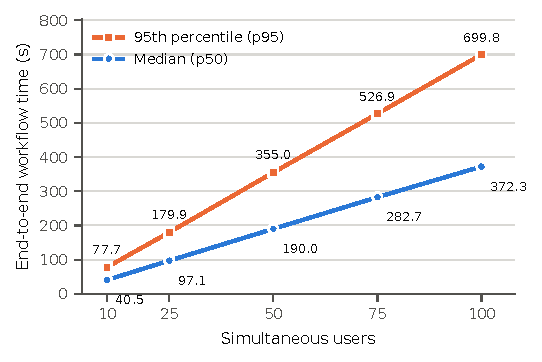
\includegraphics[width=\columnwidth]{figures/testbed/e5_latency_by_users.pdf}
  \caption{Workflow time by simultaneous users.}
  \label{fig:tb-latency}
\end{figure}
\begin{figure}[tb]
  \centering
  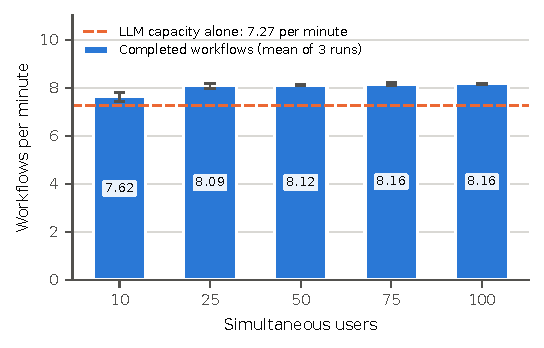
\includegraphics[width=\columnwidth]{figures/testbed/e5_throughput_by_users.pdf}
  \caption{Completed workflows per minute.}
  \label{fig:tb-throughput}
\end{figure}
The model alone, answering the 600 test cases one at a time, needs a median of 8.33~s per recommendation (9.19~s at the 95th percentile), or 7.27 recommendations per minute. It is correct on 592 of 600 cases and gives the same decision as the stored V7 evaluation for 600 of 600, which confirms that the testbed serves V7.
Fig.~\ref{fig:tb-ledger} shows the ledger on its own, with 10 to 100 transactions kept in flight. Request creation reaches 122.7 transactions per second and auditor decisions 90.6, while a single request is read 2509 times per second. The workflow runs use about 0.41 ledger transactions per second, so the ledger could take about 302 times more work than the model server lets the workflows generate.
\begin{figure}[tb]
  \centering
  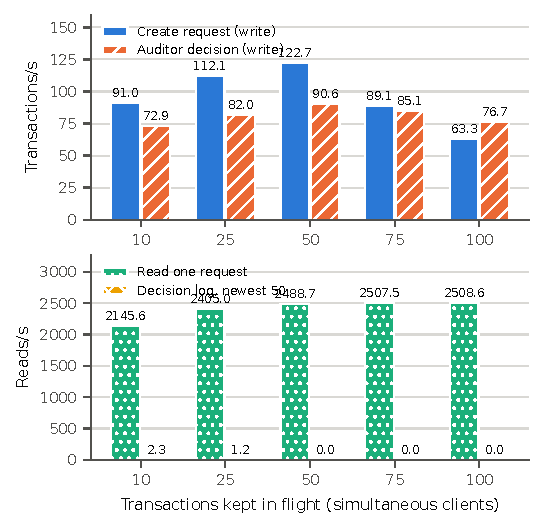
\includegraphics[width=\columnwidth]{figures/testbed/e3_throughput.pdf}
  \caption{Ledger throughput per contract function.}
  \label{fig:tb-ledger}
\end{figure}

\subsection{Resource Use and One-Hour Run}
Fig.~\ref{fig:tb-hour} shows the CPU and memory of every machine during one hour in which the 100 users send 369 requests at random times, six per minute on average. The ledger machines M1--M3 use between 0.11 and 0.18 of their three cores on average and at most 1.42~GB of their 6~GB. The model server on M5 uses 0.16 CPU cores on average, because its work runs on the GPU. Between the first and the last five minutes, the memory of each machine changes by at most 20~MB. The median workflow takes 36.5~s in the first ten minutes and 17.8~s in the last ten.
\begin{figure*}[tb]
  \centering
  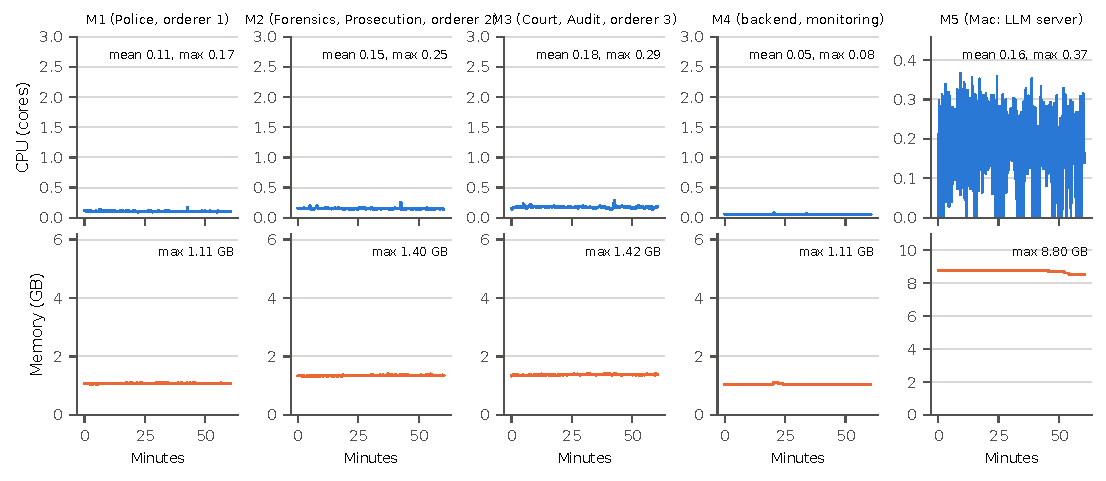
\includegraphics[width=\textwidth]{figures/testbed/e6_machines_cpu_memory.pdf}
  \caption{CPU and memory of each machine over one hour.}
  \label{fig:tb-hour}
\end{figure*}
Fig.~\ref{fig:tb-operations} counts the operations of that hour by type: 4057 of 4057 succeed (100.00\%). The workflows take a median of 24.3~s, and the recommendations agree with the policy in 358 of 369 cases.
\begin{figure}[tb]
  \centering
  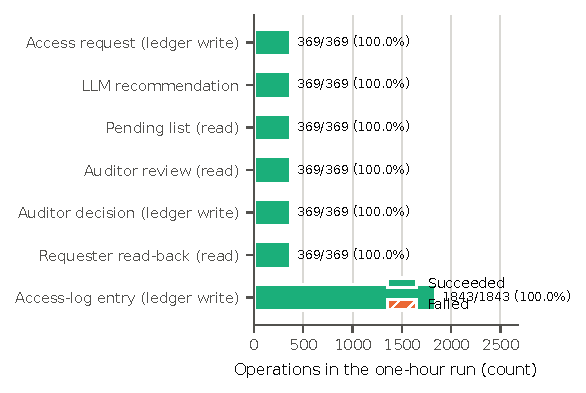
\includegraphics[width=\columnwidth]{figures/testbed/e6_operations.pdf}
  \caption{Operations in the one-hour run.}
  \label{fig:tb-operations}
\end{figure}
Fig.~\ref{fig:tb-fault} shows a separate twelve-minute run in which the Raft leader orderer is stopped for three minutes and the Court peer afterwards for three minutes. A new leader is elected 6.2~s after the leader stops. 20 of 21 workflows started while the leader was down complete, as do 17 of 17 started while the Court peer was down; two orderers still form a Raft majority, and four peers still satisfy the three-of-five endorsement rule.
\begin{figure}[tb]
  \centering
  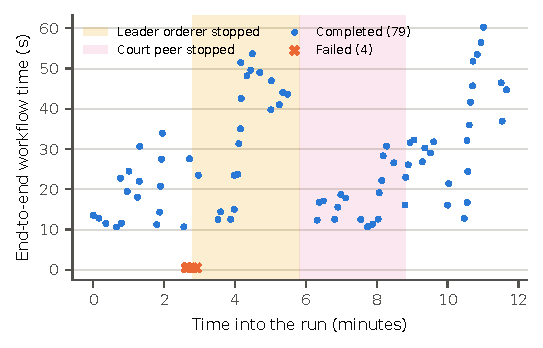
\includegraphics[width=\columnwidth]{figures/testbed/e7_fault_timeline.pdf}
  \caption{Workflows while an orderer and a peer are stopped.}
  \label{fig:tb-fault}
\end{figure}
